\chapter{Project Plan}
\label{cha:projectPlan}

%----------
\section{Task description}
The project plans are on the next pages. Tasks from the plan are described in table \ref{tab:taskDesc}. On the next page is the first plan which was released in the second week after WinLFS had been started. The second plan is a revised version.
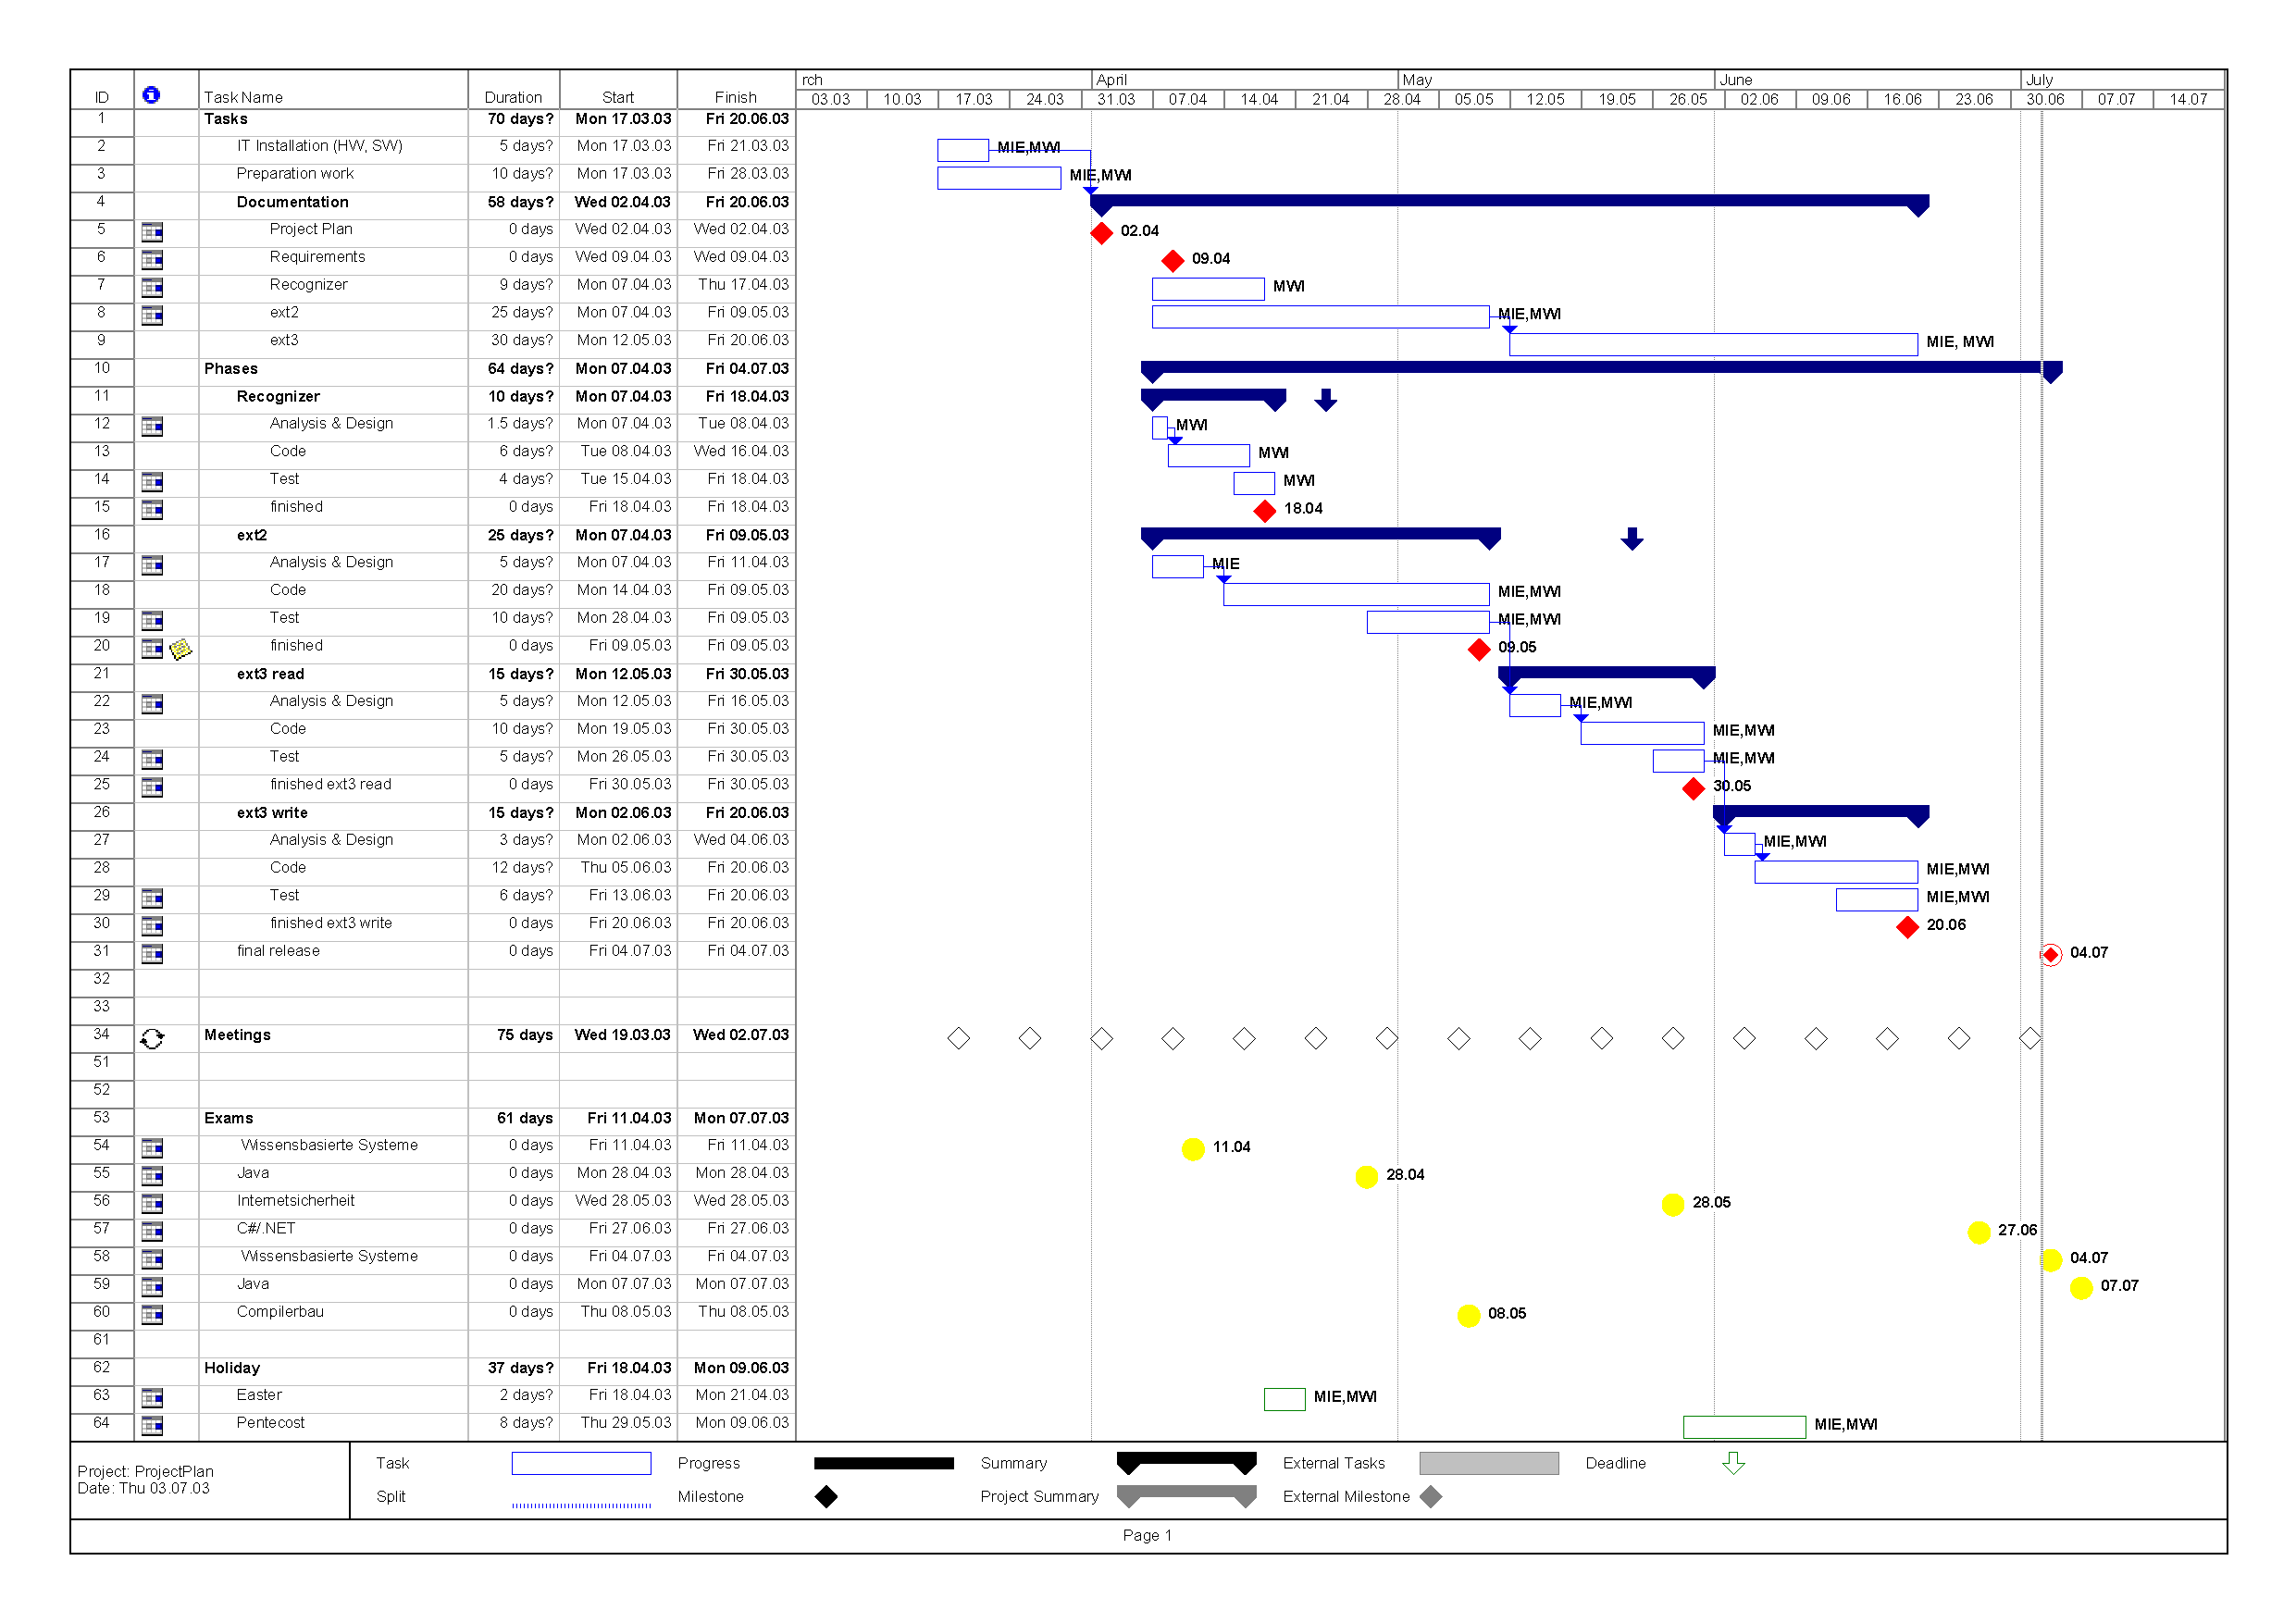
\includepdf[landscape]{./files/inc/pdf/ProjectPlan}
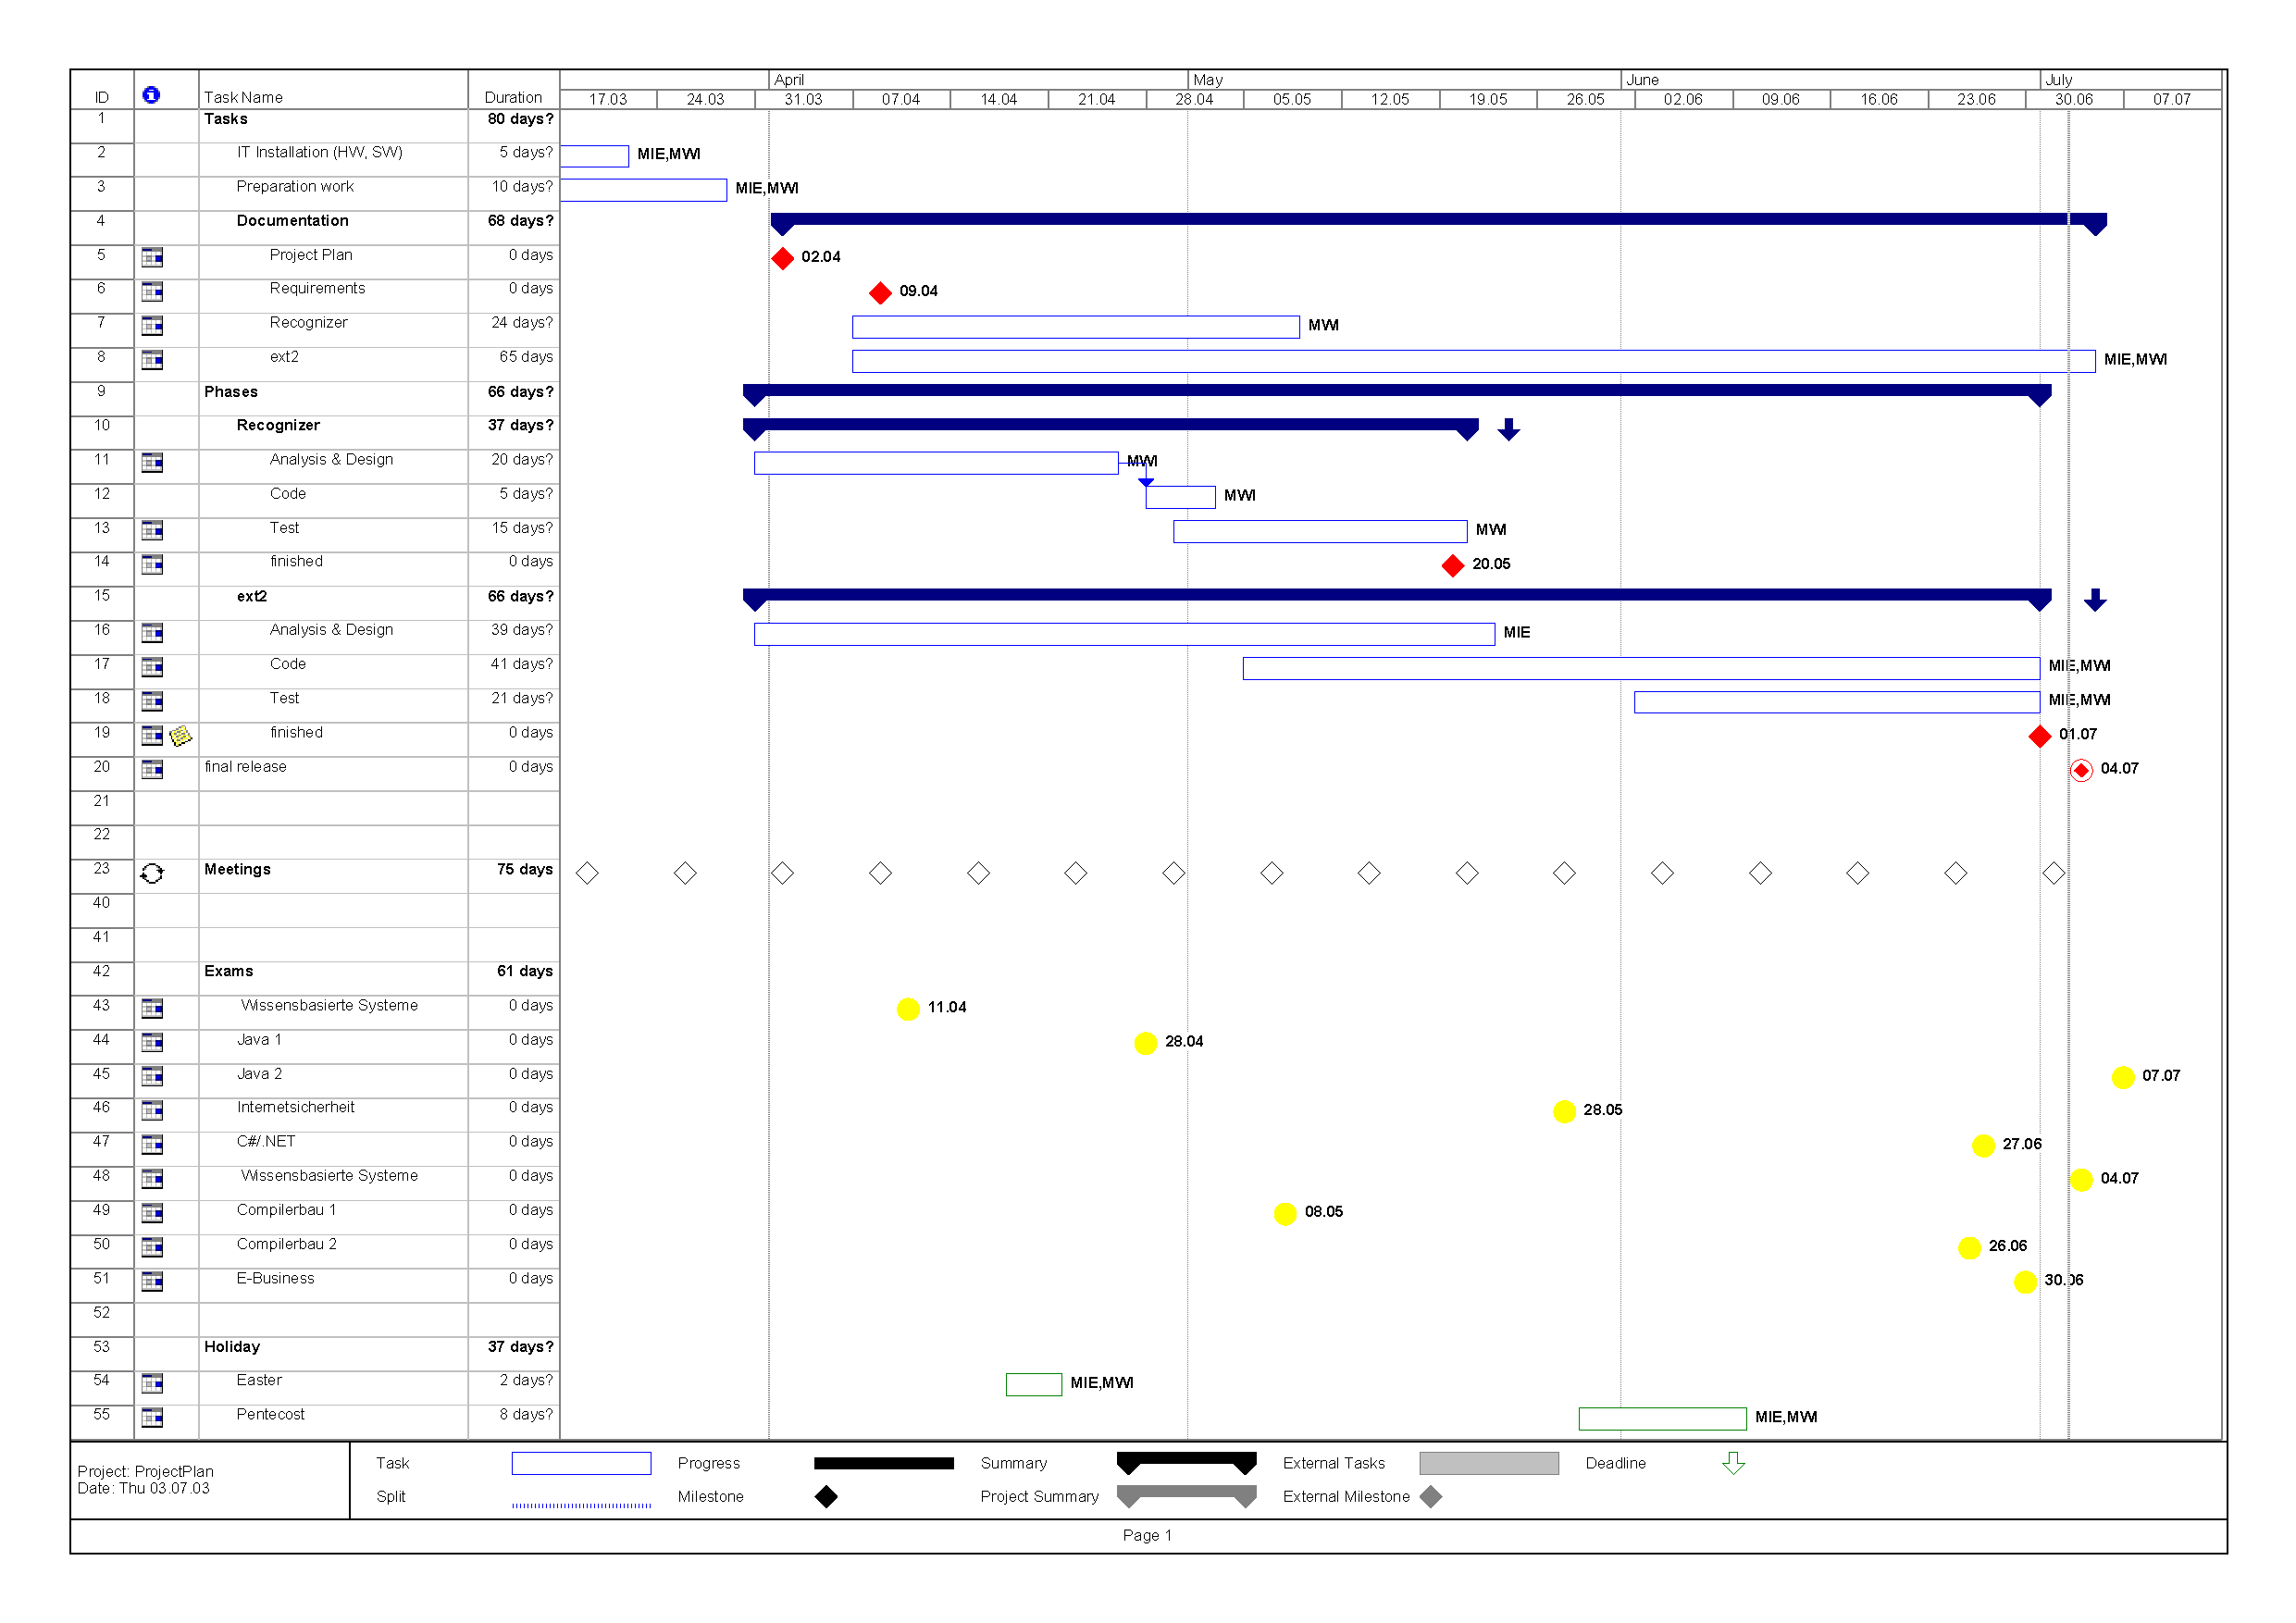
\includepdf[landscape]{./files/inc/pdf/ProjectPlan2}
\LTXtable{\linewidth}{./files/inc/tables/taskDesc}

%----------
\section{Fixed Dates}
\subsection{Meeting with Prof. E. Glatz}
\begin{tabular}{ll}
When & Wednesdays, 17.00\\
Who  & Prof. E. Glatz, Marc Winiger, Michael Egli\\
What & Define weekly goals and check them.
\end{tabular}

\subsection{Final Release}
\begin{tabular}{ll}
When & Friday, 04 July 2003\\
Who  & Prof. E. Glatz, Marc Winiger, Michael Egli\\
What & Hand Over Final Release.
\end{tabular}

\chapter{Time Variance Comparison}
\label{cha:timeVarianceComparison}
\section{Milestones}
5 milestones were planned. Each marks the end of a phase or the end of the project respectively. First we needed to set up the environment properly. This includes installation of a Linux operation system and a Windows XP installation. Additionally, we made a ghost partition on a remote host for the likely case of destroying a partition. Gladly, this has never happened. This work and the finished version of the first project plan release was milestone 1. Milestone 2 was to define all requirements and write the respective documentation. This milestones could be planned easily and the work time was within the desired scope.

Milestone 3 marks the end of the file system recognizer and milestone 4 the end of the ext2 driver development. Milestone 5 marks the final release and is the end date of this project.

As you may encounter, the second project plan differs significantly from the first one. This is due a variety of challenges we had to get over. We started the work on the recognizer parallel to the file system driver, that's why both were affected. For more information about this, read section \ref{cha:problems} further down.

\section{Planning}
\label{sec:planning}
The following table lists the estimated time for every phase and every task. We tried to estimate the needed time for every task on its own without taking into account the total amount of time for the whole project. After we had finished all estimations, we sum-up the time. The result was $445 h$, which is what we had expected before. This time variance comparison is the basis for the project plan.

\LTXtable{\linewidth}{./files/inc/tables/varianceComp}
